\chapter{Sunway系统的基本操作}\label{chap:introduction}

\section{登录}

未来Sunway官网和计算系统的登录方式可能变化,此处的登录方法仅供参考。超算中心下发了两套用户名和密码,一套用于登录VPN,一套用于登录SSH。

\subsection{登录Sunway系统SSL VPN}
\begin{enumerate}
    \item 使用IE浏览器\footnote{亲测Edge和Chrome在第一次登录时无法下载EasyConnect工具,卡在加载界面}进入神威·太湖之光官网www.nsccwx.cn;
    \item 在右上角“登录”处选择一个运营商进行登录(图\ref{fig:登录步骤1});
    \item 在弹出的警告页面\footnote{截至本章作成日2018年12月1日,太湖之光的官方网站服务器在使用自主生成的SSL证书进行https连接,这类非信任机构生成的证书会被现在的浏览器识别为不安全}中选择“详细信息”$\rightarrow$“转到此页面”(图\ref{fig:登录步骤2});
    \item 在登录界面输入俱乐部下发的VPN用户名密码进行登录(图\ref{fig:登录步骤3});
    \item 第一次登录完成后浏览器会自动下载EasyConnect工具,此工具为后续登录使用(图\ref{fig:登录步骤4}和图\ref{fig:登录步骤5})。
\end{enumerate}

再次登录时,打开第一次登录完成后自动下载的EasyConnect工具输入俱乐部下发的VPN用户名密码即可。

\subsection{SSH登录超算系统}
\begin{enumerate}
    \item 登录VPN;
    \item 在弹出的页面找到可用资源的IP地址(图\ref{fig:登录步骤6});
    \item 在命令行窗口输入“ssh [俱乐部下发的用户名]@[可用资源的IP地址]”命令进行登录\footnote{这里的用户名是SSH用户名},登录时会提示输入密码\footnote{多次登录有时会出现WARNING和登录失败,大部分情况下这都是神威系统为了安全对SSH登录验证的公钥进行定时修改所致(猜测)。这时只要删除用户目录下的C:/用户/用户名/.ssh/known\_hosts文件重新登录SSH即可(这个文件记录了所有登录过的SSH服务器的公钥,再次登录时会进行公钥比对,如果不符则登录失败)},此处密码为SSH登录密码(图\ref{fig:登录步骤7});
    \item 出现bash界面说明登录成功(图\ref{fig:登录步骤8})。
\end{enumerate}

\begin{figure}[!htbp]
    \centering
    \begin{subfigure}[b]{0.49\textwidth}
      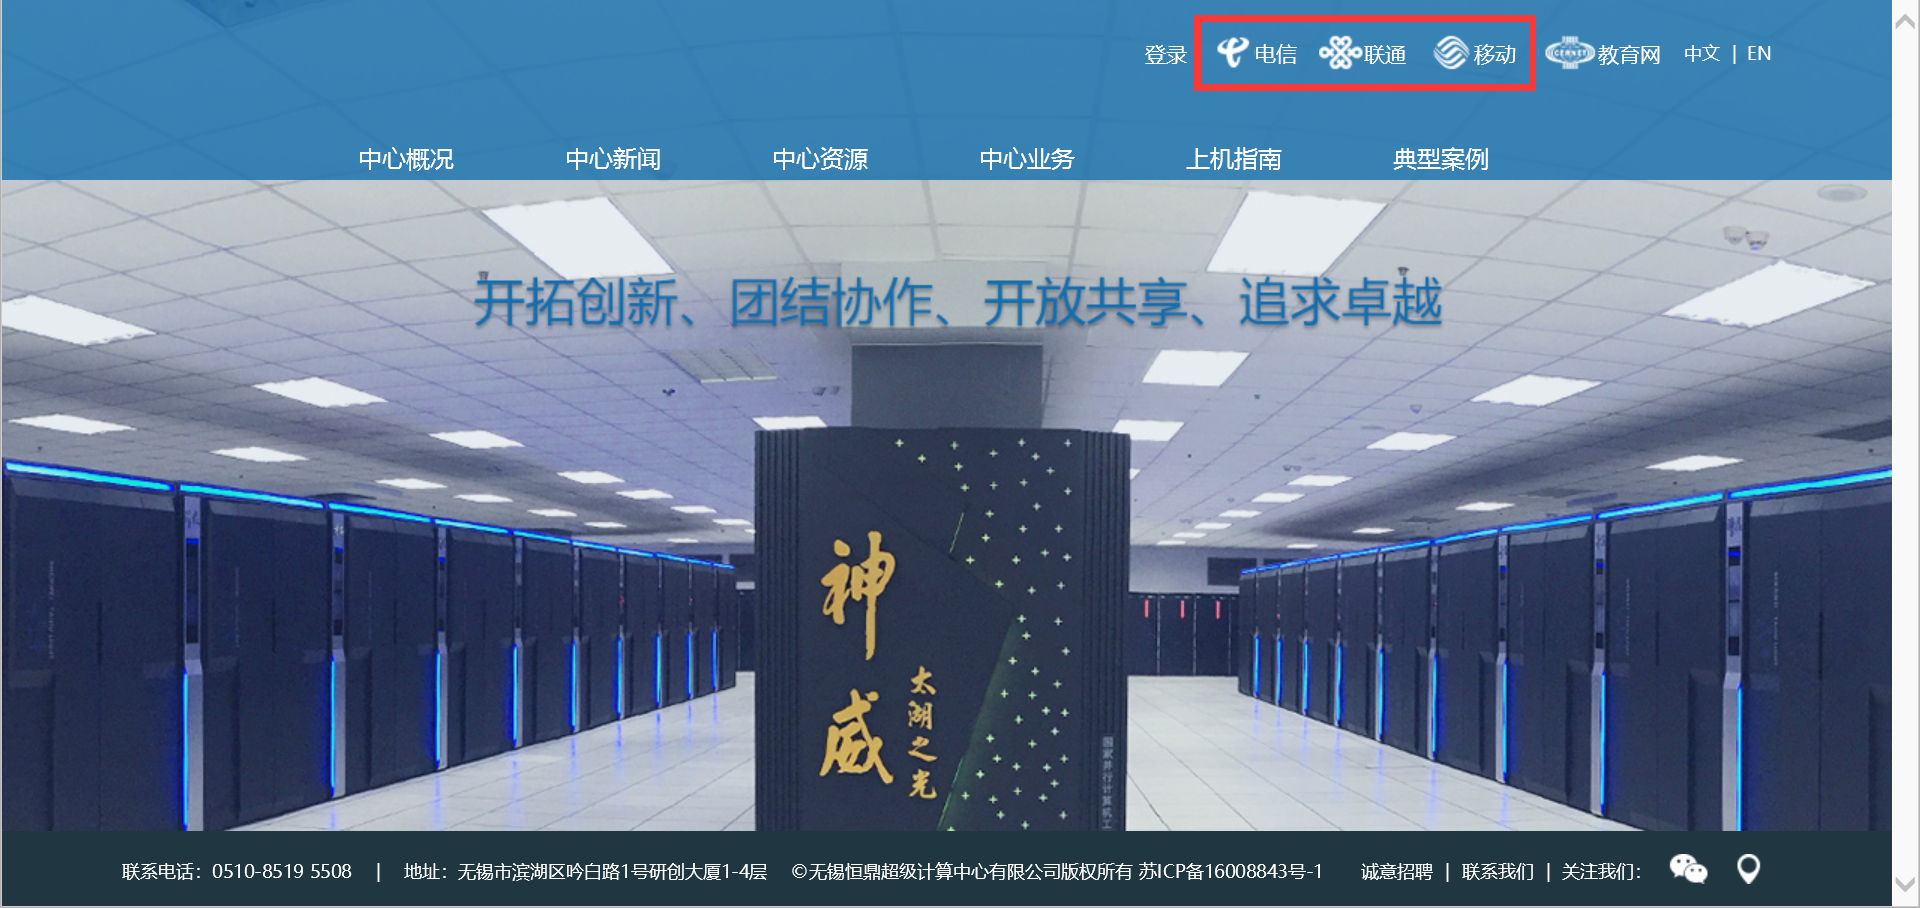
\includegraphics[width=\textwidth]{Login/1.png}
      \caption{官网主页}
      \label{fig:登录步骤1}
    \end{subfigure}%
    ~% add desired spacing
    \begin{subfigure}[b]{0.49\textwidth}
      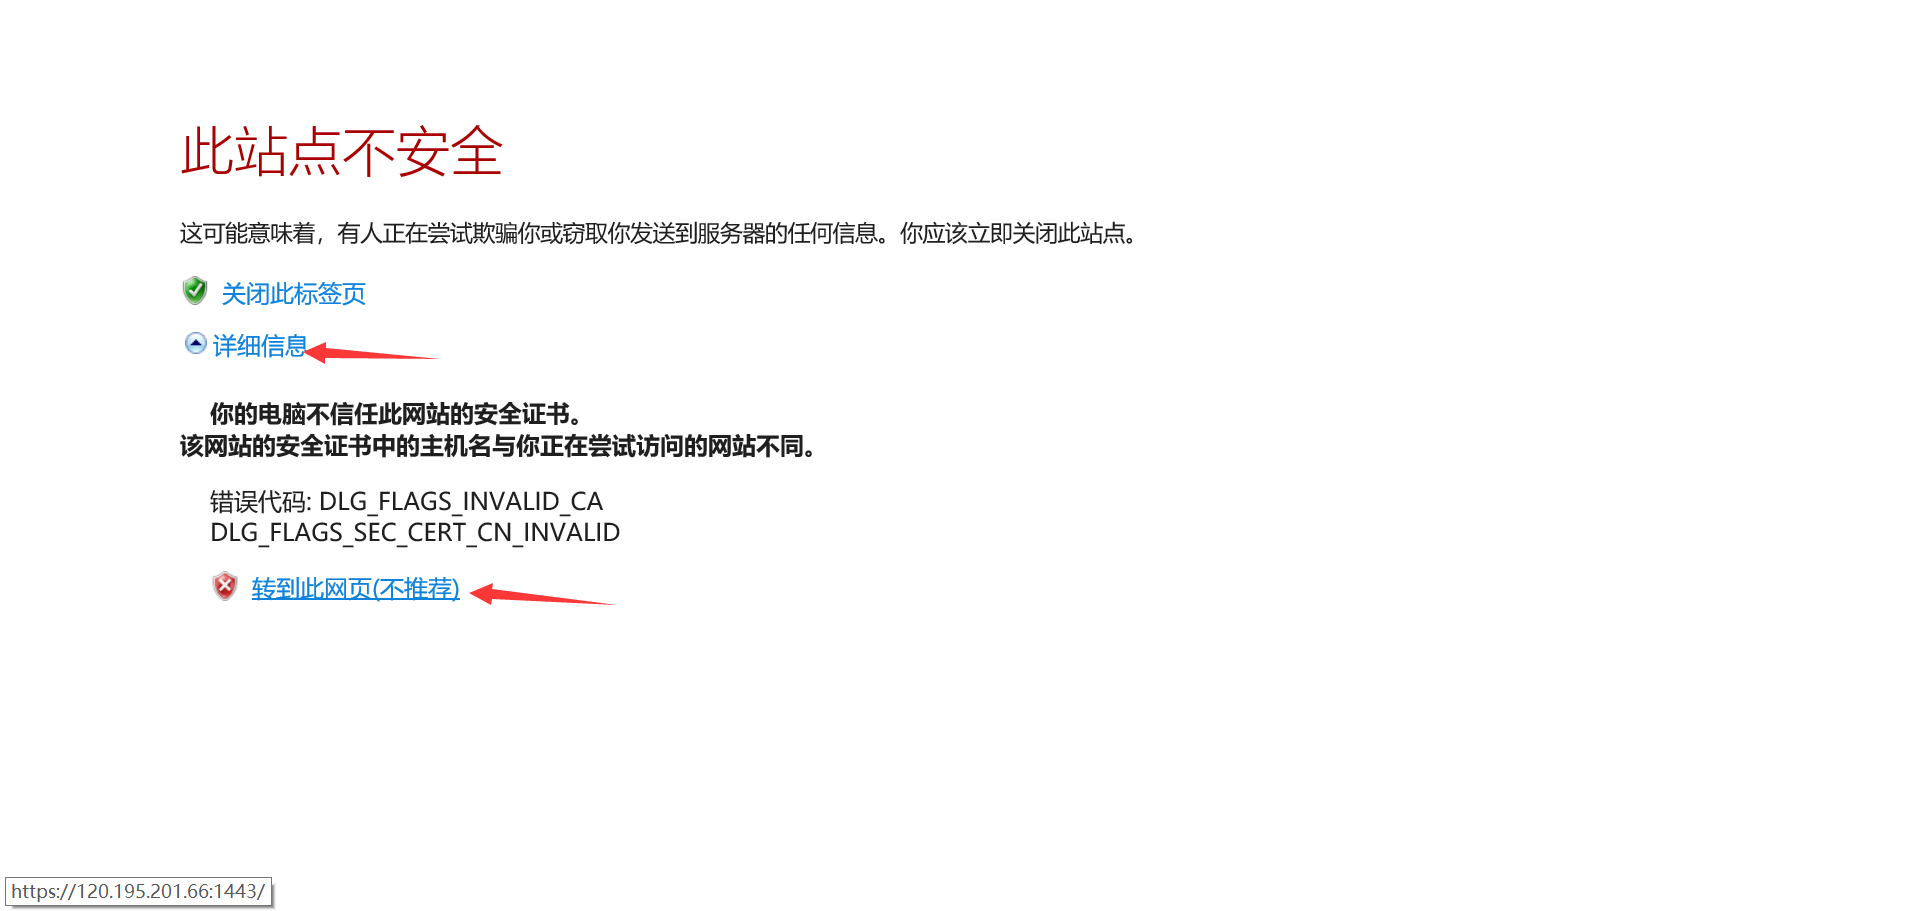
\includegraphics[width=\textwidth]{Login/2.png}
      \caption{进入登录页面}
      \label{fig:登录步骤2}
    \end{subfigure}
    \\% line break
    \begin{subfigure}[b]{0.49\textwidth}
      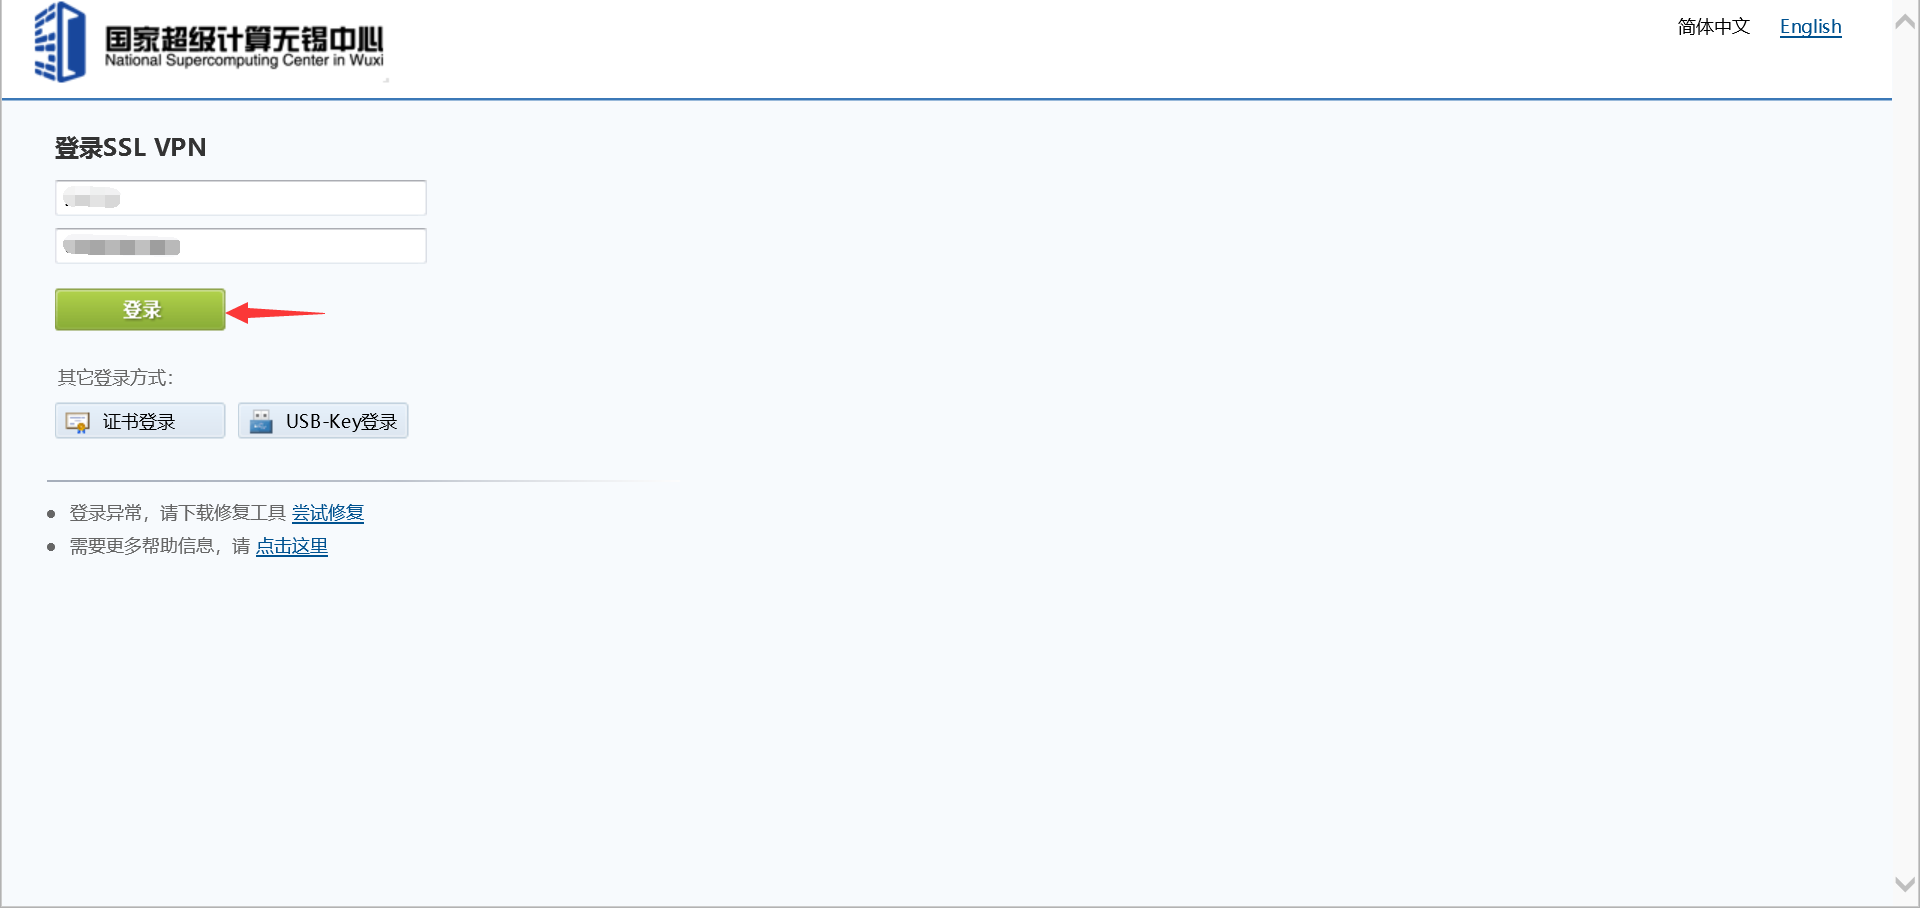
\includegraphics[width=\textwidth]{Login/3.png}
      \caption{登录VPN}
      \label{fig:登录步骤3}
    \end{subfigure}%
    ~% add desired spacing
    \begin{subfigure}[b]{0.49\textwidth}
      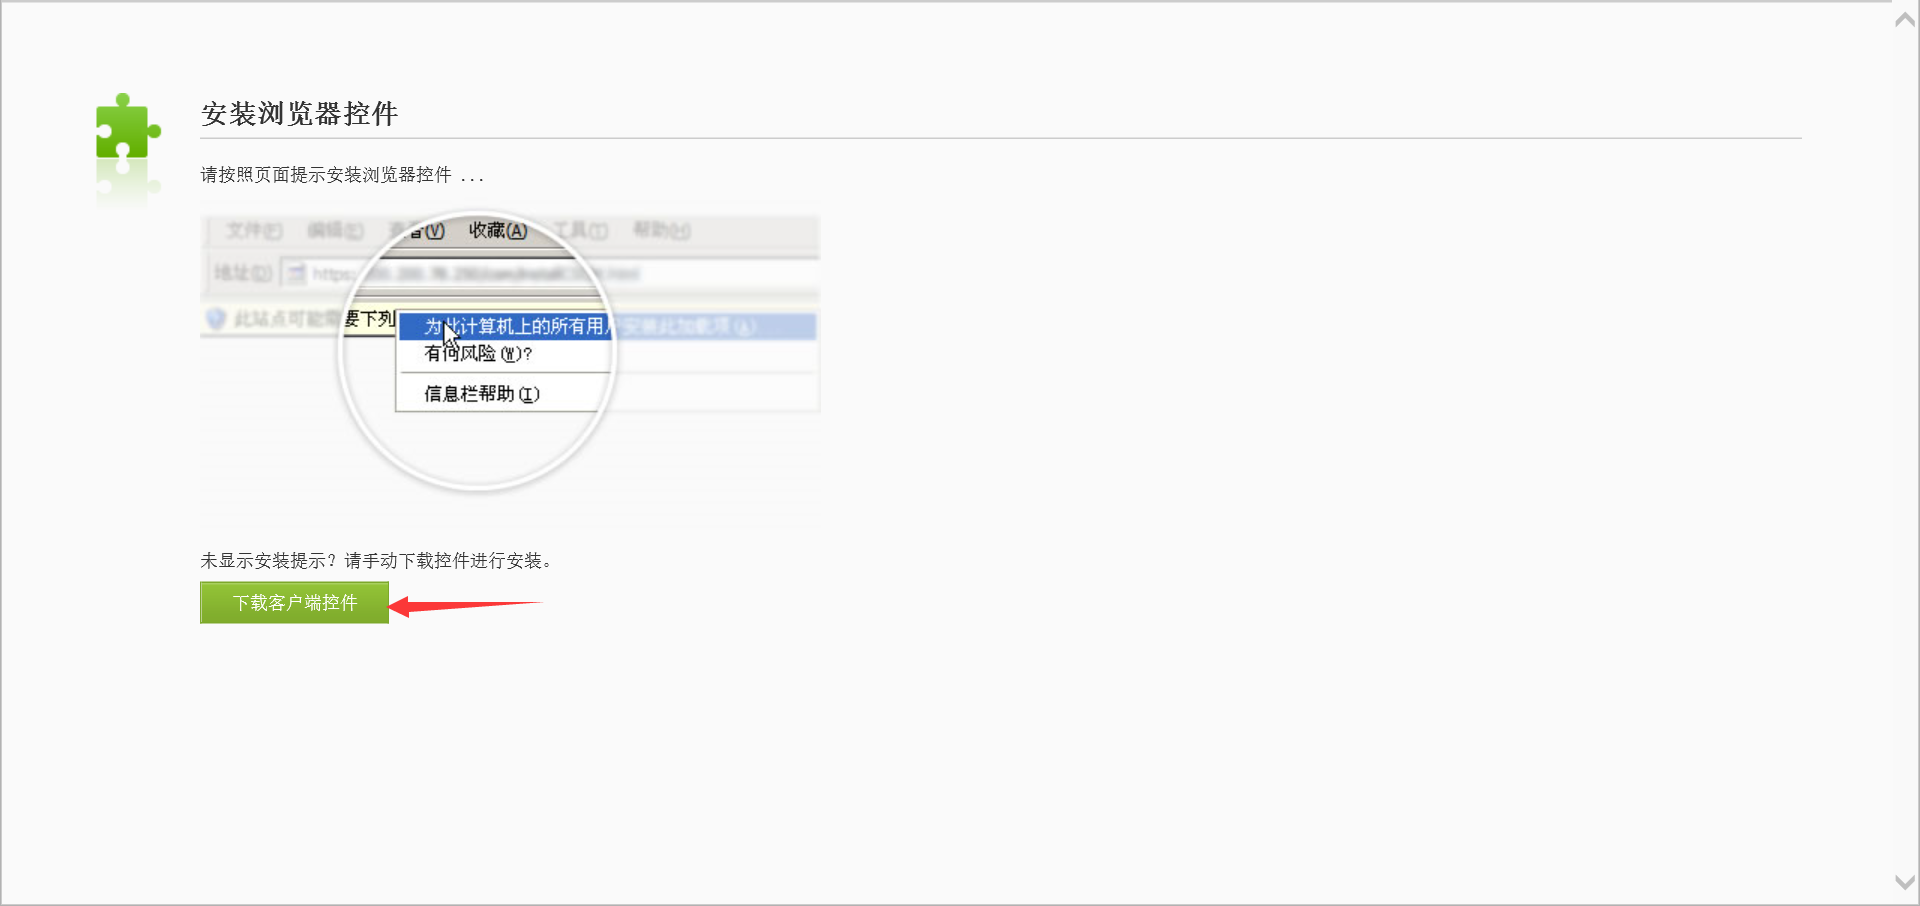
\includegraphics[width=\textwidth]{Login/4.png}
      \caption{下载EasyConnect}
      \label{fig:登录步骤4}
    \end{subfigure}
    \\% line break
    \begin{subfigure}[b]{0.49\textwidth}
      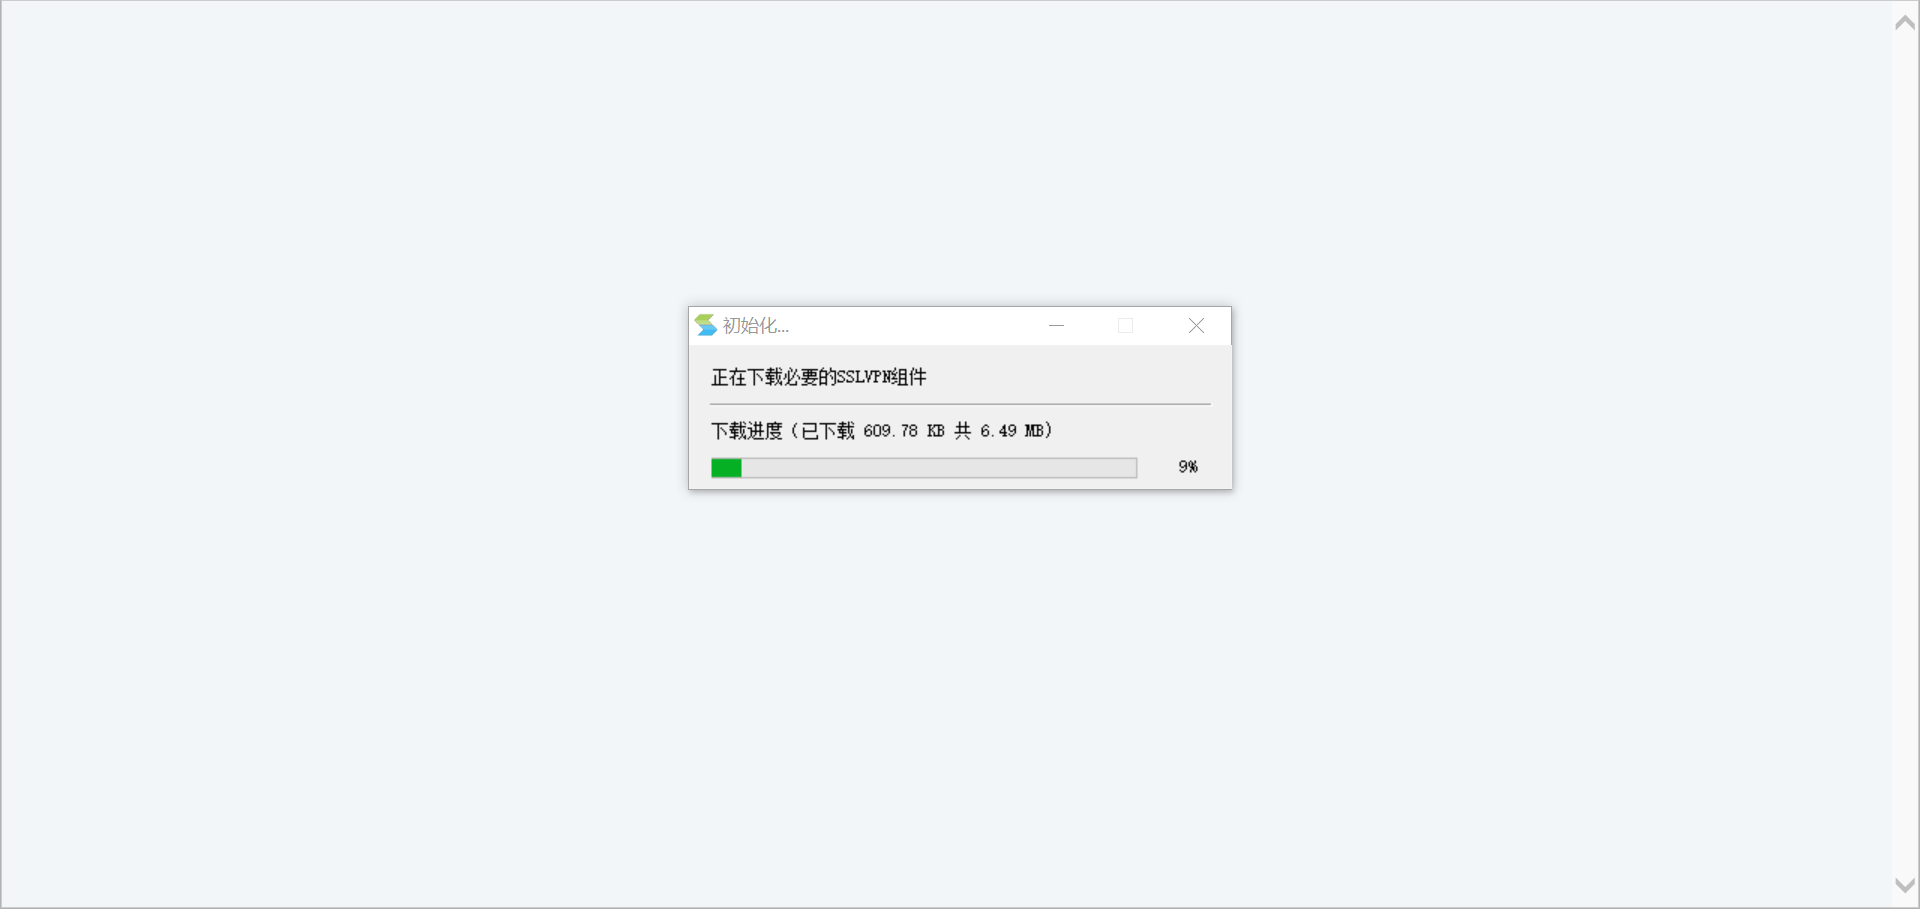
\includegraphics[width=\textwidth]{Login/5.png}
      \caption{安装EasyConnect}
      \label{fig:登录步骤5}
    \end{subfigure}%
    ~% add desired spacing
    \begin{subfigure}[b]{0.49\textwidth}
      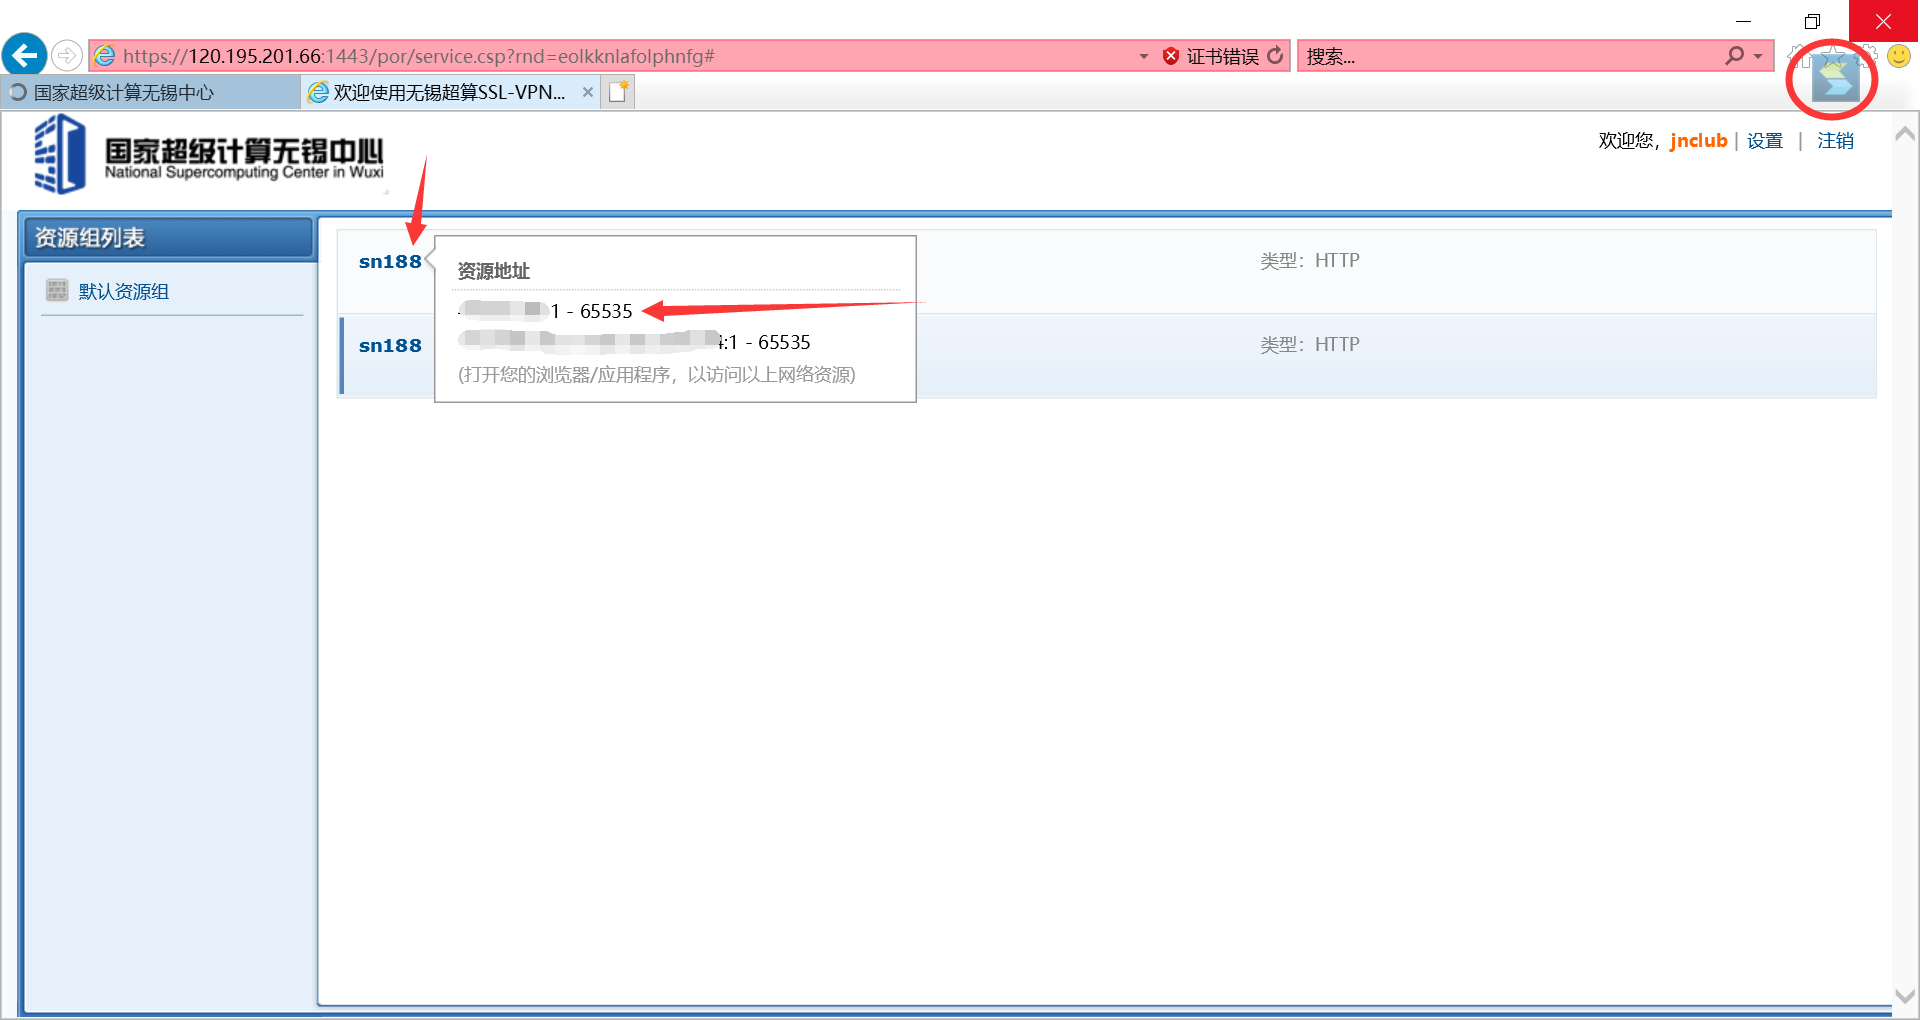
\includegraphics[width=\textwidth]{Login/6.png}
      \caption{找可用资源}
      \label{fig:登录步骤6}
    \end{subfigure}
    \\% line break
    \begin{subfigure}[b]{0.49\textwidth}
      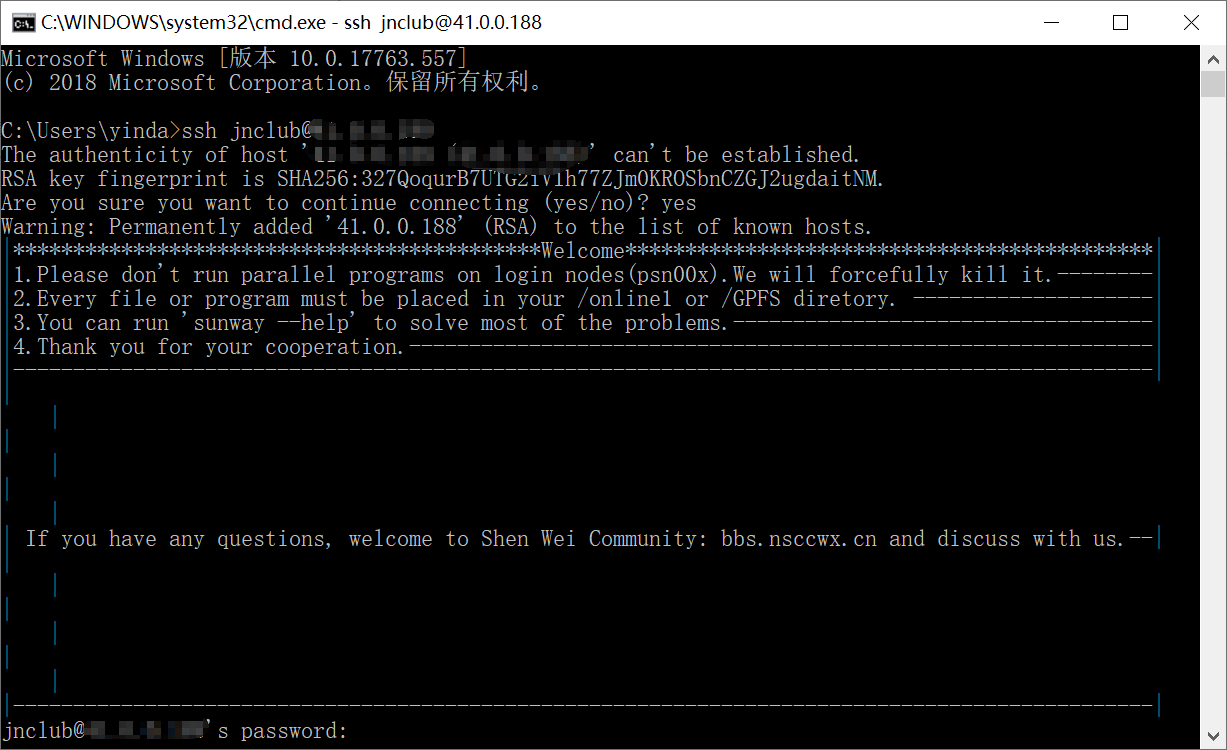
\includegraphics[width=\textwidth]{Login/7.png}
      \caption{用可用资源IP登录SSH}
      \label{fig:登录步骤7}
    \end{subfigure}%
    ~% add desired spacing
    \begin{subfigure}[b]{0.49\textwidth}
      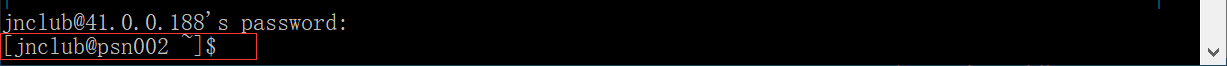
\includegraphics[width=\textwidth]{Login/8.png}
      \caption{登录成功}
      \label{fig:登录步骤8}
    \end{subfigure}
    \caption{超算系统登录流程}
    \label{fig:oaspl}
\end{figure}

\section{第一个程序:矩阵相加}
矩阵计算是所有并行计算的基础,第一个并行程序以矩阵相加程序为例,介绍在单个SW26010处理器上编程时Sunway编译器和Athread的一些基本操作。矩阵相加程序的要求非常简单:将两个64x2048的矩阵相加。

\subsection{单个SW26010处理器并行计算流程}\label{section:并行计算的基本流程}
正如前言中所说,每个SW26010芯片中都包含4个处理器,每个处理器有1个主核和64个从核,第一个程序的编写将着眼于在一个处理器上的编程,程序只使用1个主核和64个从核。

\begin{enumerate}
	\item 运行于主核上的主程序启动N个并行执行的线程(N$\leq$64),每个线程都在一个从核上执行;
	\item 在并行执行的线程中,每个线程都从主存储中\textbf{不同的位置}取出数据放入从核各自的局部存储中\footnote{在一般的并行编程中都有在并行线程中获取线程编号的方法,并行线程即通过线程编号计算出自己要从哪个位置取数\label{footnote:取数据说明}}\footnote{从主存储中取出数据放入从核的局部存储使用称作DMA(Direct Memory Access,直接内存存取)的方法,DMA运行独立于主核和从核,可以在主核和从核进行计算的同时传输数据,在基于传输的并行优化方面尤其有用\label{footnote:DMA}};
	\item 从核在自己的局部存储上进行计算;
	\item 从核计算完成后,都分别将计算结果放回到主存储中后结束自身的线程;
	\item 在从核运行过程中主程序进行其他其他操作并等待所有从核线程结束;
	\item 所有的从核线程结束(从核函数退出)之后,主程序进行下一步并行操作或结束。
\end{enumerate}

\subsection{相关Athread函数}
下面是矩阵相加程序中使用到的并行函数相关必要知识的介绍,更加详细的描述见《编译手册》第五章“加速线程库”。
\subsubsection{在主核中调用的Athread函数}
\begin{enumerate}
	\item athread\_init()核组初始化,在所有athread操作之前都要进行调用;
	\item athread\_set\_num\_threads()设置下一次并行操作启动的线程总数,如果不设置此项值则下一次并行操作(athread\_spawn)启动64个线程;
	\item athread\_spawn([函数指针],[传入参数])在从核上启动并行线程,[函数指针]为指向从核函数入口的指针(从核函数名),且该指针需要在文件开头使用一个Athread库中的宏“extern SLAVE\_FUN(从核函数名)()”进行声明;[传入参数]为向每个从核函数传递的实参该参数会在运行时传递到每个并行从核函数线程中;
	\item athread\_join()等待所有从核线程结束,程序执行到此函数时会阻塞直到所有从核线程结束才会执行下一步;
	\item athread\_halt()关闭线程组流水线,在所有并行操作完成之后才能调用此函数,在程序结束时调用,调用后运算核心将无法在本进程中再次使用。
\end{enumerate}

\subsubsection{在从核中调用的Athread函数}
\begin{enumerate}
	\item athread\_get\_id()获取线程逻辑标号,一般在从核程序中通过此函数的值判断应该从主存储的哪个位置取数据;
	\item athread\_get([传输模式],[源地址],[目的地址],[数据量],[回答字地址],[],[],[])通过DMA(见注\ref{footnote:DMA})方法从主存中读取数据写入从核局部存储。各形参含义为:
	\begin{itemize}
		\item 传输模式:DMA传输命令模式,本例程中只涉及使用PE\_MODE;
        \item 源地址:要传输的数据在主核中的地址(在主核程序中的变量名)。对于数组形式的数据,此处填数组变量的首地址,就像下面这样\footnote{这里的取数位置即是从核函数要从何处取数的标志(见注\ref{footnote:取数据说明}),该值一般由athread\_get\_id()获取到的线程逻辑标号计算得出}。多维数组的取址方法以此类推。
		\begin{lstlisting}
&源数组名[取数位置]//一维数组首地址位置
&源数组名[取数位置1][取数位置2]//二维数组首地址位置
        \end{lstlisting}
        上面写出的源数组名数组名需要在从核程序开头进行“extern”声明,如下所示。
		\begin{lstlisting}
extern 数据类型 源数组名;//文件开头声明主核中的某个数组
		\end{lstlisting}
		\item 目的地址:从主存中取得的数据放入局部存储的哪个地址(变量)中。对于数组形式的数据其写法和源地址相同,且数组名需要在从核函数文件开头进行“\_\_thread\_local”声明,如下所示。
		\begin{lstlisting}
extern 数据类型 源数组名;//文件开头声明主核中的某个数组
		\end{lstlisting}
		\item 数据量:从源地址开始读取多少\textbf{字节}数据到局部存储(目的地址)中。对于数组形式的数据,此参数的值为[要读多少个数]*[此数组的数据类型占多少字节]\footnote{实测在太湖之光的编译系统中,int型和float型占4个字节,long型和double型占8个字节}。
		\item 回答字地址:当athread\_get数据传输完成时,回答字地址中的值加1。多个athread\_get同时运行可以共用一个回答字,每个athread\_get运行结束时都会使回答字地址中的值加1。一般在等待athread\_get传输完成的地方会有“while([回答字]!=[共用此回答字的athread\_get函数个数]);”。回答字变量在从核函数文件开头以“\_\_thread\_local volatile”声明。
		\item 本例程不涉及最后三个参数。
	\end{itemize}
\end{enumerate}


\subsection{并行编程思路}\label{subsec:并行编程思路}
并行编程程序分主核和从核两个程序流程,请理解上文所述的各函数的作用并理解下列流程后自行编写程序。参考程序见附录\ref{apdx:第一个程序}。
\newline 主核程序:
\begin{enumerate}
    \item 生成两个64x2048矩阵;
    \item athread\_init()初始化;
    \item athread\_spawn()启动64个从核线程,每个线程处理每个64X2048矩阵中的2048个数;
    \item athread\_join()等待线程全部结束;
    \item athread\_halt()关闭线程流水线;
    \item 输出结果,退出程序。
\end{enumerate}
从核程序:
\begin{enumerate}
    \item athread\_get\_id()获取线程逻辑标号;
    \item athread\_get()根据线程逻辑标号从主核程序变量中取得要用的数据,每个线程取在两个64x2048矩阵中各取2048个数;
    \item 计算相加结果;
    \item athread\_put()将结果写回主核程序变量中;
    \item 退出程序。
\end{enumerate}

\section{程序的编译}
“神威 · 太湖之光”系统的编译环境有两种,一种是服务于高速计算系统的编译环境,即SW26010搭建的神威主系统;另一种服务于辅助计算系统,该系统是常见的Intel X86 CPU + GPU结构服务器。这里只介绍高速计算系统环境下的程序编译。本节主要内容来自《优化手册》2.5节“编译环境”。

\subsection{Sunway程序编译简介}
目前的“神威 · 太湖之光”系统支持的编程语言主要包括C语言(C99)、C++语言(C++03和C++11)和Fortran(Fortran2003),其中C++目前还不能编译从核程序。

神威系统的C语言编译器指令为“sw5cc”,编译模式分为主核和从核两种\footnote{正如前言中所说,异构计算使用不同类型指令集和体系架构的计算单元组成系统,因此在编译程序时主核和从核使用的编译器并不相同},编译主核程序的指令为:
\begin{lstlisting}
sw5cc -host [选项] 文件名.c
\end{lstlisting}
编译从核的指令为:
\begin{lstlisting}
sw5cc -slave [选项] 文件名.c
\end{lstlisting}
主核程序和从核程序编译完成后,则使用下面这个命令进行混合链接生成可执行程序:
\begin{lstlisting}
sw5cc -hybrid [选项] 主核文件名.o 从核文件名.o
\end{lstlisting}

本章只介绍编译器的基本使用方法,不过多涉及编译器的编译选项,详细了解编译选项可见《优化手册》表格2-2。

\subsection{用命令行编译程序}\label{subsec:用命令行编译程序}
假设在\ref{subsec:并行编程思路}节编写的主核程序源文件名“master\_arrAdd.c”、从核程序源文件名“slave\_arrAdd.c”,则可以输入下面这三条指令对源文件进行编译和链接:
\begin{enumerate}
  \item 编译主核,-c选项表示为每个源文件生成一个.o文件但不进行链接
\begin{lstlisting}
sw5cc -host -c master_arrAdd.c
\end{lstlisting}
  \item 编译从核
\begin{lstlisting}
sw5cc -slave -c slave_arrAdd.c
\end{lstlisting}
  \item 链接,-o arrAdd选项表示输出的可执行文件名为“arrAdd”
\begin{lstlisting}
sw5cc -hybrid master_arrAdd.o slave_arrAdd.o -o arrAdd
\end{lstlisting}
\end{enumerate}

编译完成后即可在当前目录下看到一个可执行文件“arrAdd”。接下来介绍运行这个可执行文件的方法。

\section{程序的运行}
和上一节介绍的编译环境一样,神威系统的运行也分高速计算系统运行和辅助计算系统运行两种,这里也只介绍程序在高速计算系统中的运行,主要内容来自《优化手册》2.6节“作业提交”。

\subsection{Sunway程序运行简介}
“神威 · 太湖之光”的高速计算系统计算资源由一个作业管理系统进行管理,其本质是一个队列。在高速计算系统上运行的程序称为“作业”,要运行某个作业时,将这个作业提交到作业管理系统的队列中,作业管理系统按照先进先出方式取出队列中的作业放到计算节点上运行。

俱乐部目前持有的账号可以向免费的开发调试计算队列提交作业:高速计算系统的q\_sw\_expr和辅助计算系统的q\_x86\_expr。这两个队列中每个作业的最长运行时间为60分钟,最大并行规模为64。

\subsection{用命令行运行程序}
神威系统提交作业的指令为“bsub”,其指令选项内容丰富,此处不一一展开,详细的选项可见《优化手册》2.6.2节,这里只介绍几个常见的选项。

使用“bsub”指令运行\ref{subsec:用命令行编译程序}中编译完成的可执行程序“arrAdd”,可键入如下指令:
\begin{lstlisting}
bsub -I -b -q q_sw_expr -n 1 -cgsp 64 ./arrAdd
\end{lstlisting}
指令选项解释:
\begin{itemize}
  \item -I:使作业输出在当前窗口;
  \item -q q\_sw\_expr:将作业提交到q\_sw\_expr计算队列;
  \item -b:指定从核栈位于局部存储,该选项使得从核程序先全部读入从核局部再运行,可以减少主从核数据传输的次数,对于并行计算的速度提升非常重要;
  \item -n 1:指定程序要用的核组个数为1;
  \item -cgsp 64:指定每个核组内要用的从核个数为64,由于一个SW26010一个核组只有64个从核,因此该值不能大于64。该选项即影响程序中athread\_spawn()生成的从核线程的个数;
  \item ./arrAdd:要执行的可执行文件位置。
\end{itemize}

若使用附录\ref{apdx:第一个程序}中的程序,在程序执行完成后可得到并行和非并行计算的结果与时间对比。

\section{总结}
\subsection{知识点概括}
本章主要介绍了在神威系统编写程序的流程和必须要知道的一些基本操作,内容可大致概括为图\ref{fig:Chap_Intro}。

\begin{figure}[!htbp]
  \centering
  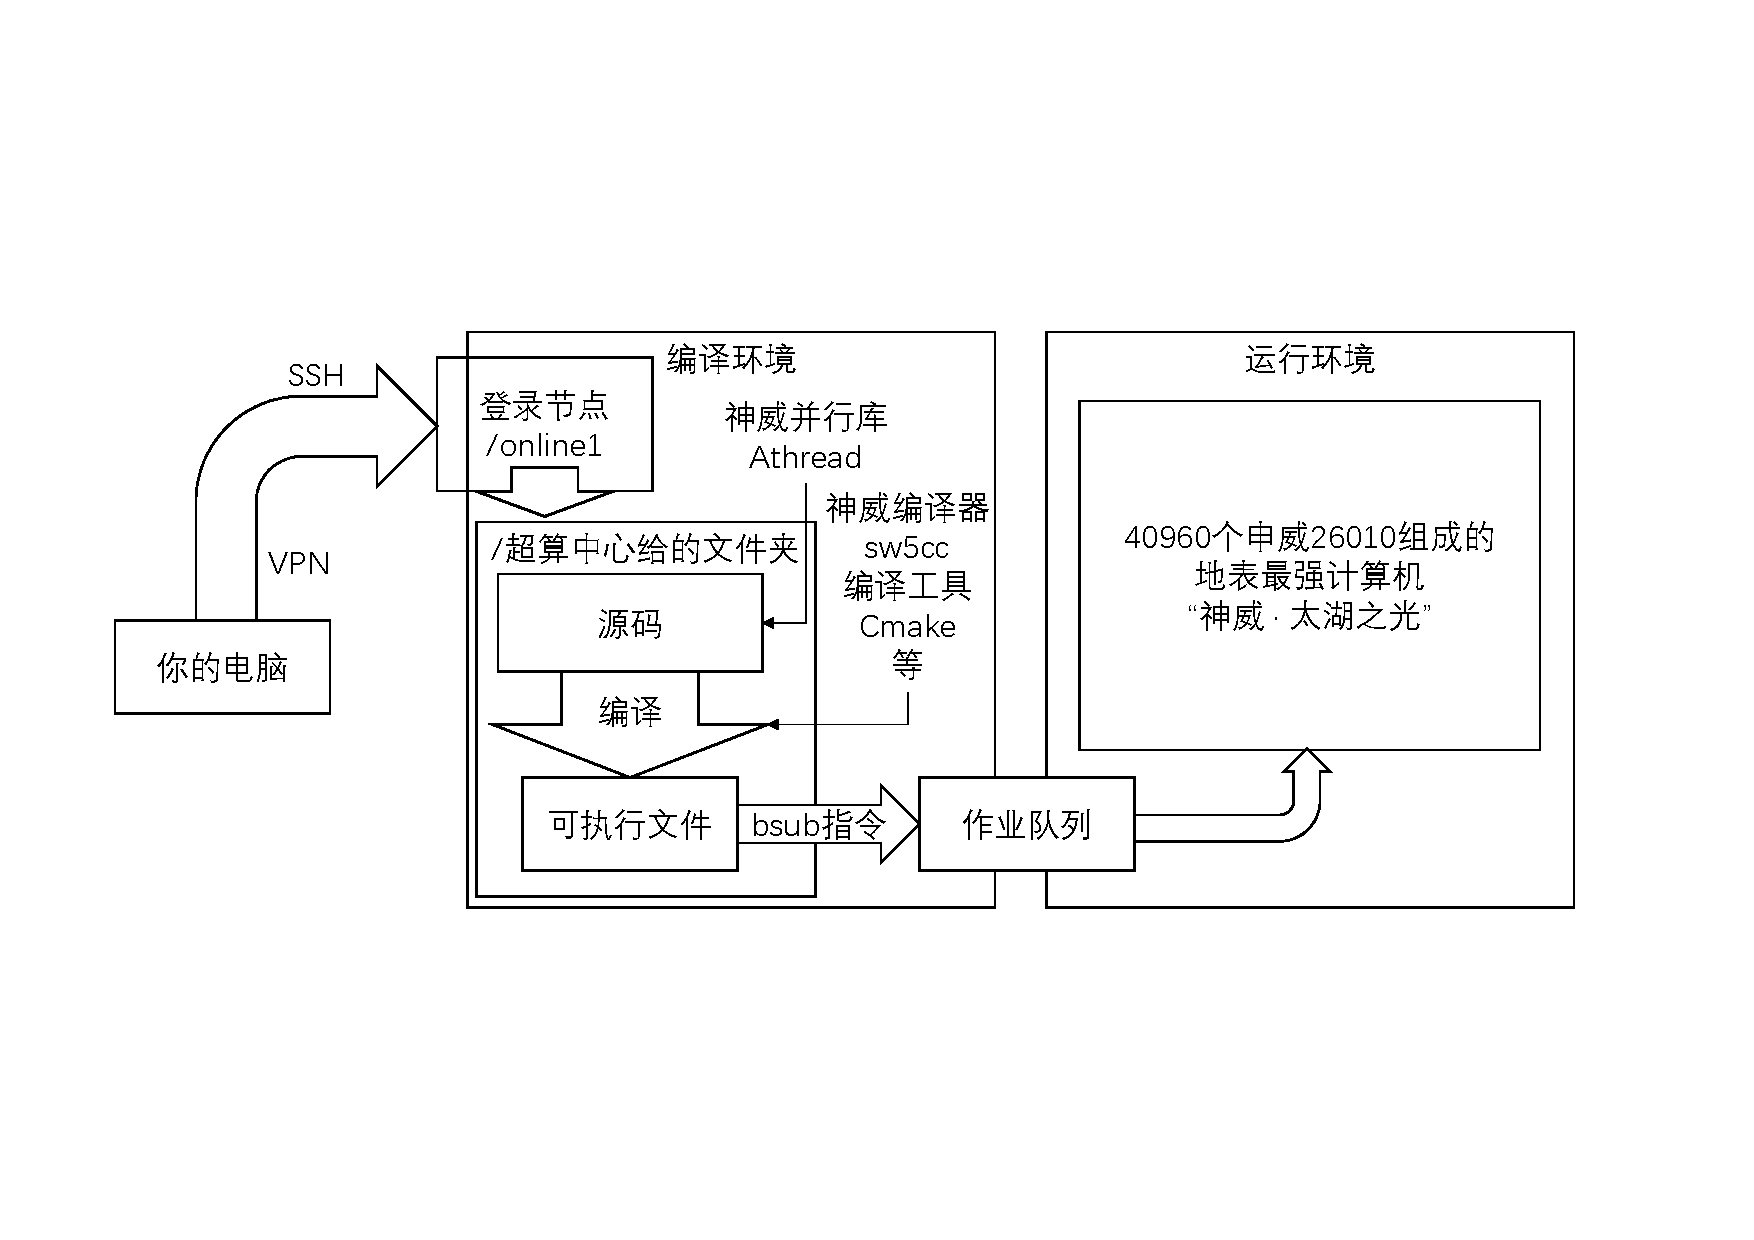
\includegraphics[width=\textwidth]{Chap_Intro}
  \caption{第一章的知识点概括}
  \label{fig:Chap_Intro}
\end{figure}

\subsection{练习}
\begin{itemize}
  \item 用Athread实现并行的矩阵减法;
  \item 用Athread实现并行的矩阵乘法。
\end{itemize}